\section{Curvature-Driven Surface Hopping Algorithms}\label{sec:curvature_driven_surface_hopping_algorithms}
\textit{Commentary on: \fullcite{10.1021/acs.jctc.5c01176}}

The second published work of this thesis focuses on curvature-driven surface hopping algorithms from article \textit{Curvature-Driven Nonadiabatic Dynamics without Explicit Nonadiabatic Couplings} in \textit{Journal of Chemical Theory and Computation}. All simulations on model potentials in this work were performed using custom-built \textsc{Zinq} package.\supercite{10.5281/zenodo.18386143}

When performing nonadiabatic dynamics simulations, one has several options how to treat the nonadiabatic transitions between electronic states. The most common approach is to use surface hopping methods, where classical nuclear trajectories evolve on \glspl{pes} and can hop between them based on certain criteria. The most widely used surface hopping method is the \gls{fssh} method, described in Sec.~\ref{sec:fewest_switches}, which relies on the calculation of \gls{tdc} to propagate the electronic wavefunction in adiabatic basis. Details about the \gls{tdc} can be found in Sec.~\ref{sec:time_derivative_coupling} and the adiabatic basis is described in Sec.~\ref{sec:adiabatic_vs_diabatic_representation}. From quantum-chemical calculations, the \gls{tdc} is usually obtained using \gls{nacv} (Eq.~\eqref{eq:tdc_nacv}) that are computationally expensive to calculate and not available for all electronic structure methods. The question arises whether it is possible to perform nonadiabatic dynamics simulations without the need to calculate \gls{nacv} at all.

One of the fairly known approaches to avoid the calculation of \gls{tdc} is to use the \gls{lzsh}, described in depth in Sec.~\ref{sec:landau_zener}, which estimates the hopping probabilities based on the exact solution of a two-level system with linearly varying diabatic energies and constant diabatic coupling. The \gls{lzsh} method has been successfully applied in various nonadiabatic dynamics simulations, but it is not as popular as the \gls{fssh} method due to its theoretical limitations and fairly recent applications to simulations in adiabatic basis. Since most of the quantum-dynamical codes already provide \gls{fssh} implementation, it would be beneficial to have a method that can be easily incorporated into existing \gls{fssh} frameworks without the need to calculate \gls{nacv} from \textit{ab initio} methods.

The study presented in this article aims to evaluate the performance of the newly proposed curvature-driven $\kappa$\gls{fssh} method in comparison to the traditional \gls{fssh} and \gls{lzsh} methods. The theory behind the $\kappa$\gls{fssh} method is described in detail in Sec.~\ref{sec:baeck_an}. The surface hopping methods are tested on several one-dimensional model systems, including single avoided crossing, three-state crossing and models exhibiting trivial crossings. After the one-dimensional models, the study applies the algorithm to more realistic systems as 8-dimensional model of uracil cation or nonadiabatic dynamics of stilbene, azobenzene or cyclobutanone. In the simulations, the quantities of interest are the state populations and the magnitude of the \gls{tdc}. The populations obtained from the surface hopping methods are compared to the numerically exact quantum dynamics results (Sec.~\ref{sec:split_operator_method}), while the \gls{tdc} values are compared to those calculated from the \gls{npi} algorithm described in Sec.~\ref{sec:norm_preserving_interpolation}. The study also introduces a modified version of the $\kappa$\gls{fssh} method, called $\lambda$\gls{fssh}, which should theoretically be more accurate in predicting the \gls{tdc} values (Eq.~\eqref{eq:lambda_tdc}).

Since the standard \gls{lzsh} algorithm is strictly formulated for two-level systems, applying it to environments with three-state crossings requires theoretical extensions. To address this, the study introduces two generalized multistate variants: the maximum curvature version (\gls{lzsh}$_{\symrm{maxcurv}}$) and the nearest state version (\gls{lzsh}$_{\symrm{nearest}}$). When a multistate crossing is identified, the \gls{lzsh}$_{\symrm{maxcurv}}$ algorithm computes transition probabilities only to the state exhibiting the maximum second derivative of the energy gap ($\ddot{Z}_{ik}$), operating on the physical premise that strongly interacting states will exhibit the sharpest curvature. Alternatively, the \gls{lzsh}$_{\symrm{nearest}}$ variant restricts population transfer strictly to the energetically closest state. Both variants are critically evaluated alongside the curvature-driven \gls{fssh} schemes.
\subsection{Simulations on Model Systems}
The results from the simulations on a single avoided crossing model in Fig.~\ref{fig:curvature_single_avoided_crossing} show that the $\kappa$\gls{fssh} already performs significantly worse than the traditional \gls{fssh} and \gls{lzsh} methods in terms of state populations. Inspecting the \gls{tdc} in this case reveals that the $\kappa$\gls{fssh} method produces a narrower peak compared to the reference \gls{npi} values, which likely contributes to the poorer performance in state populations.
\begin{figure}[!ht]
\centering
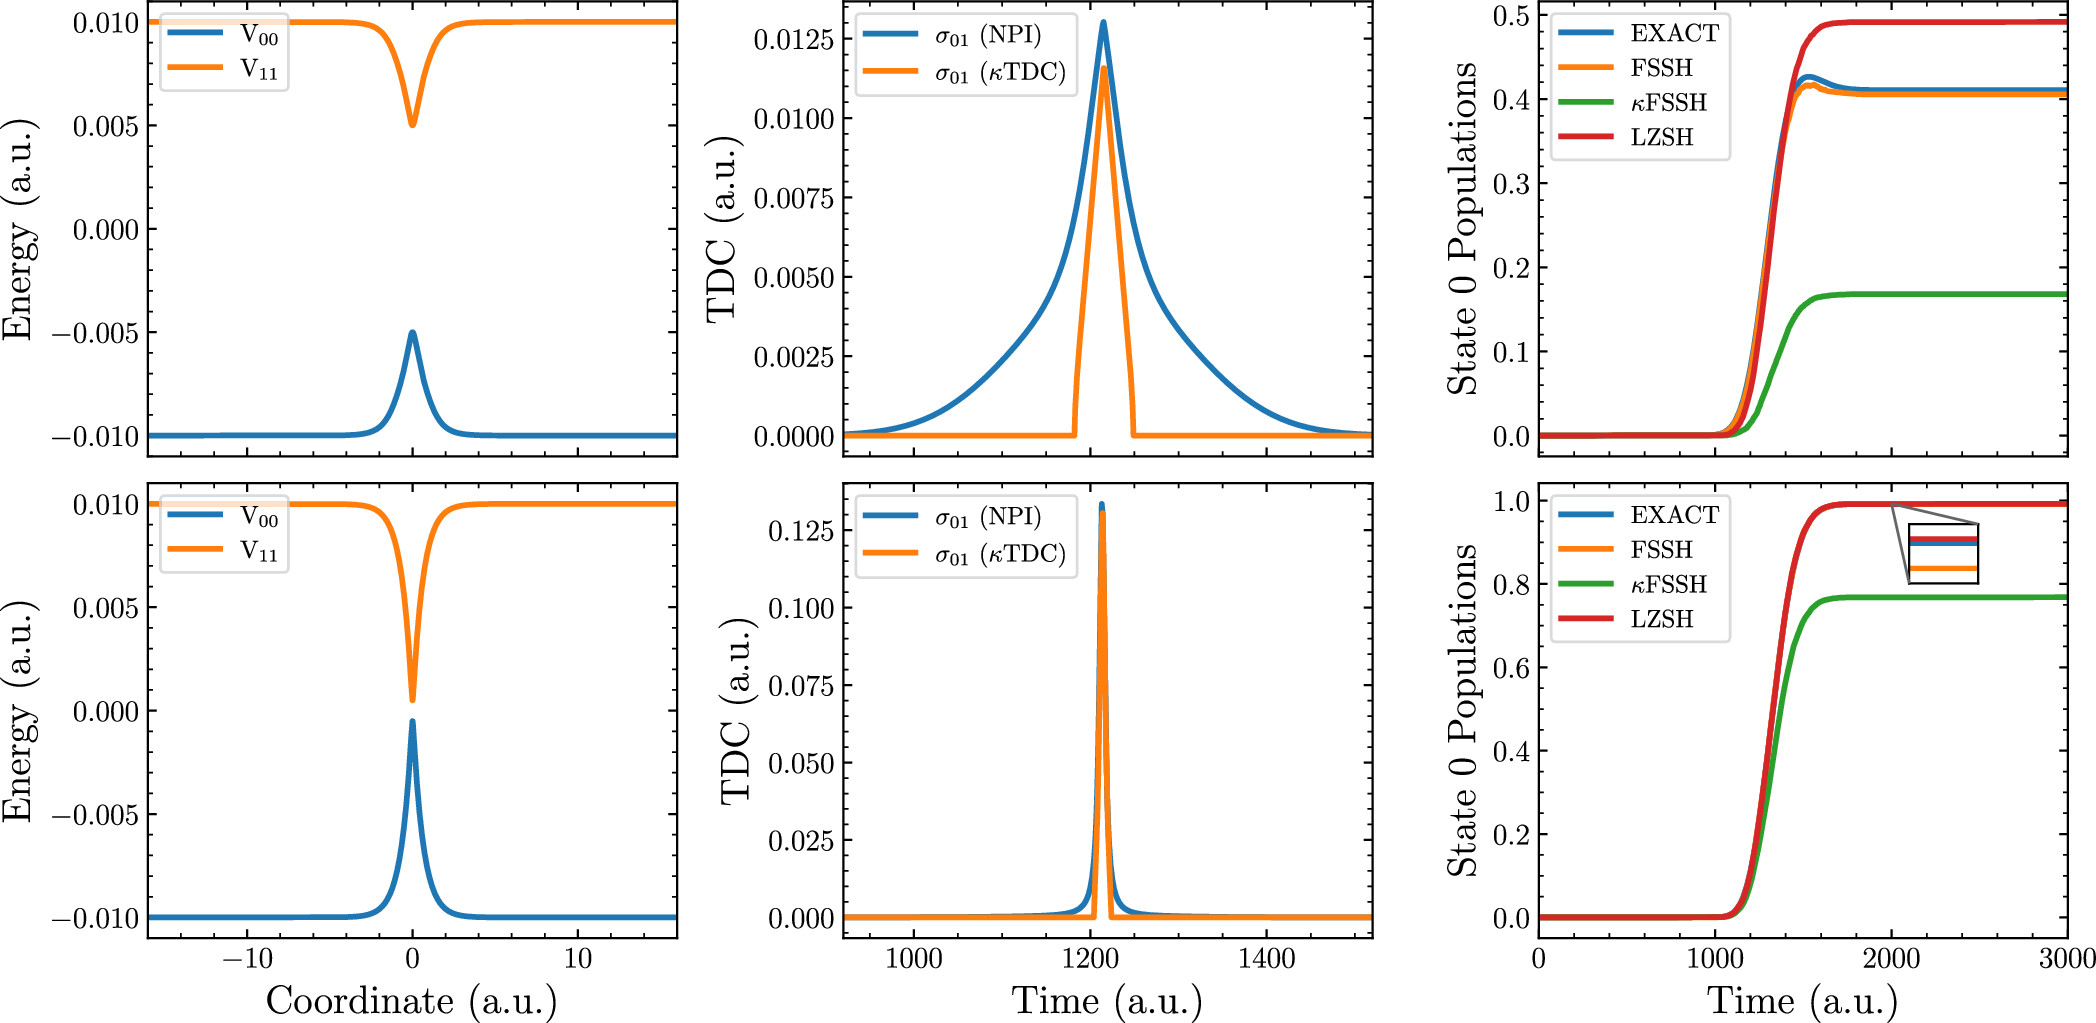
\includegraphics[width=\linewidth]{parts/02-Original_Research_and_Contributions/chapters/02-Primary_Scientific_Contributions/sections/images/images_large_ct5c01176_0002}
\caption{Nonadiabatic dynamics simulations on Tully’s Simple Avoided Crossing potential defined using two different sets of diabatic coupling constants. Reproduced from Ref.~\cite{10.1021/acs.jctc.5c01176} under \href{https://creativecommons.org/licenses/by/4.0}{CC BY 4.0}.}
\label{fig:curvature_single_avoided_crossing}
\end{figure}
In the three-state crossing model (Fig.~\ref{fig:curvature_three-state_crossing}), the performance of the $\kappa$\gls{fssh} method is even more unsatisfactory. The fundamental flaw of the curvature-driven approach becomes apparent here: because $\kappa$\gls{fssh} relies solely on the adiabatic energy gap ($Z_{ik}$) and its temporal derivatives, it assigns non-zero \gls{tdc} values between any states that are energetically close, even if their wavefunctions are strictly orthogonal and no physical coupling exists. For instance, while the reference \gls{npi} method correctly predicts zero coupling between states 0 and 2, $\kappa$\gls{fssh} artificially forces population transfer between them, leading to unphysical trajectory outcomes.
\begin{figure}[!ht]
\centering
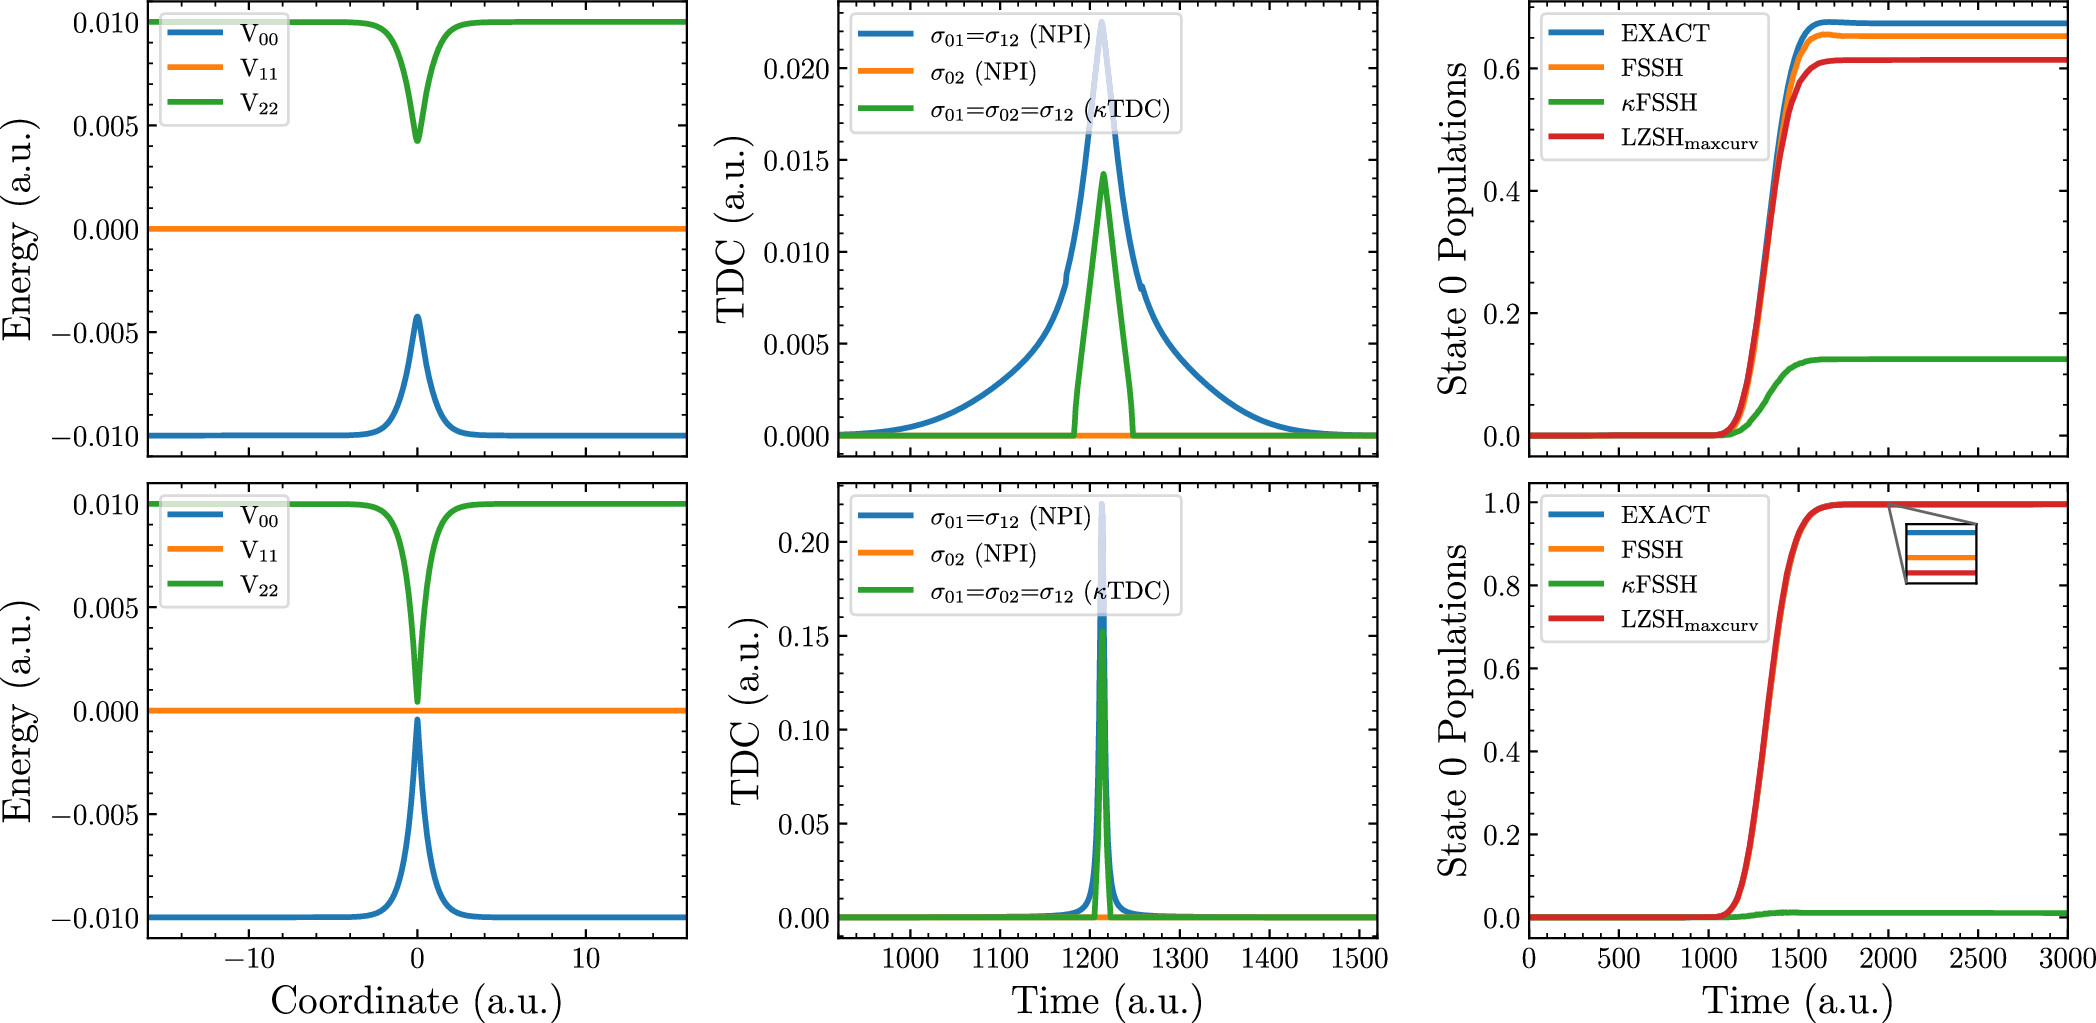
\includegraphics[width=\linewidth]{parts/02-Original_Research_and_Contributions/chapters/02-Primary_Scientific_Contributions/sections/images/images_large_ct5c01176_0003}
\caption{Nonadiabatic dynamics simulations on three-state crossing potential defined using two different sets of diabatic coupling constants. Reproduced from Ref.~\cite{10.1021/acs.jctc.5c01176} under \href{https://creativecommons.org/licenses/by/4.0}{CC BY 4.0}.}
\label{fig:curvature_three-state_crossing}
\end{figure}
Moving on to the trivial crossing models (Fig.~\ref{fig:curvature_trivial_crossing}), the $\kappa$\gls{fssh} method again fails to reproduce the correct state populations, while the traditional \gls{fssh} and \gls{lzsh} methods perform without issues. At a trivial crossing, the true \gls{nacv} theoretically approaches a singularity (a Dirac delta function), necessitating a complete 100\% population transfer. However, investigating the \gls{tdc} values reveals that the analytical form of the $\kappa$\gls{fssh} and $\lambda$\gls{fssh} approximations fundamentally caps the maximum coupling magnitude, producing a finite, broadened peak instead of a singularity. This insufficient coupling magnitude traps residual population in the excited state.
\begin{figure}[!ht]
\centering
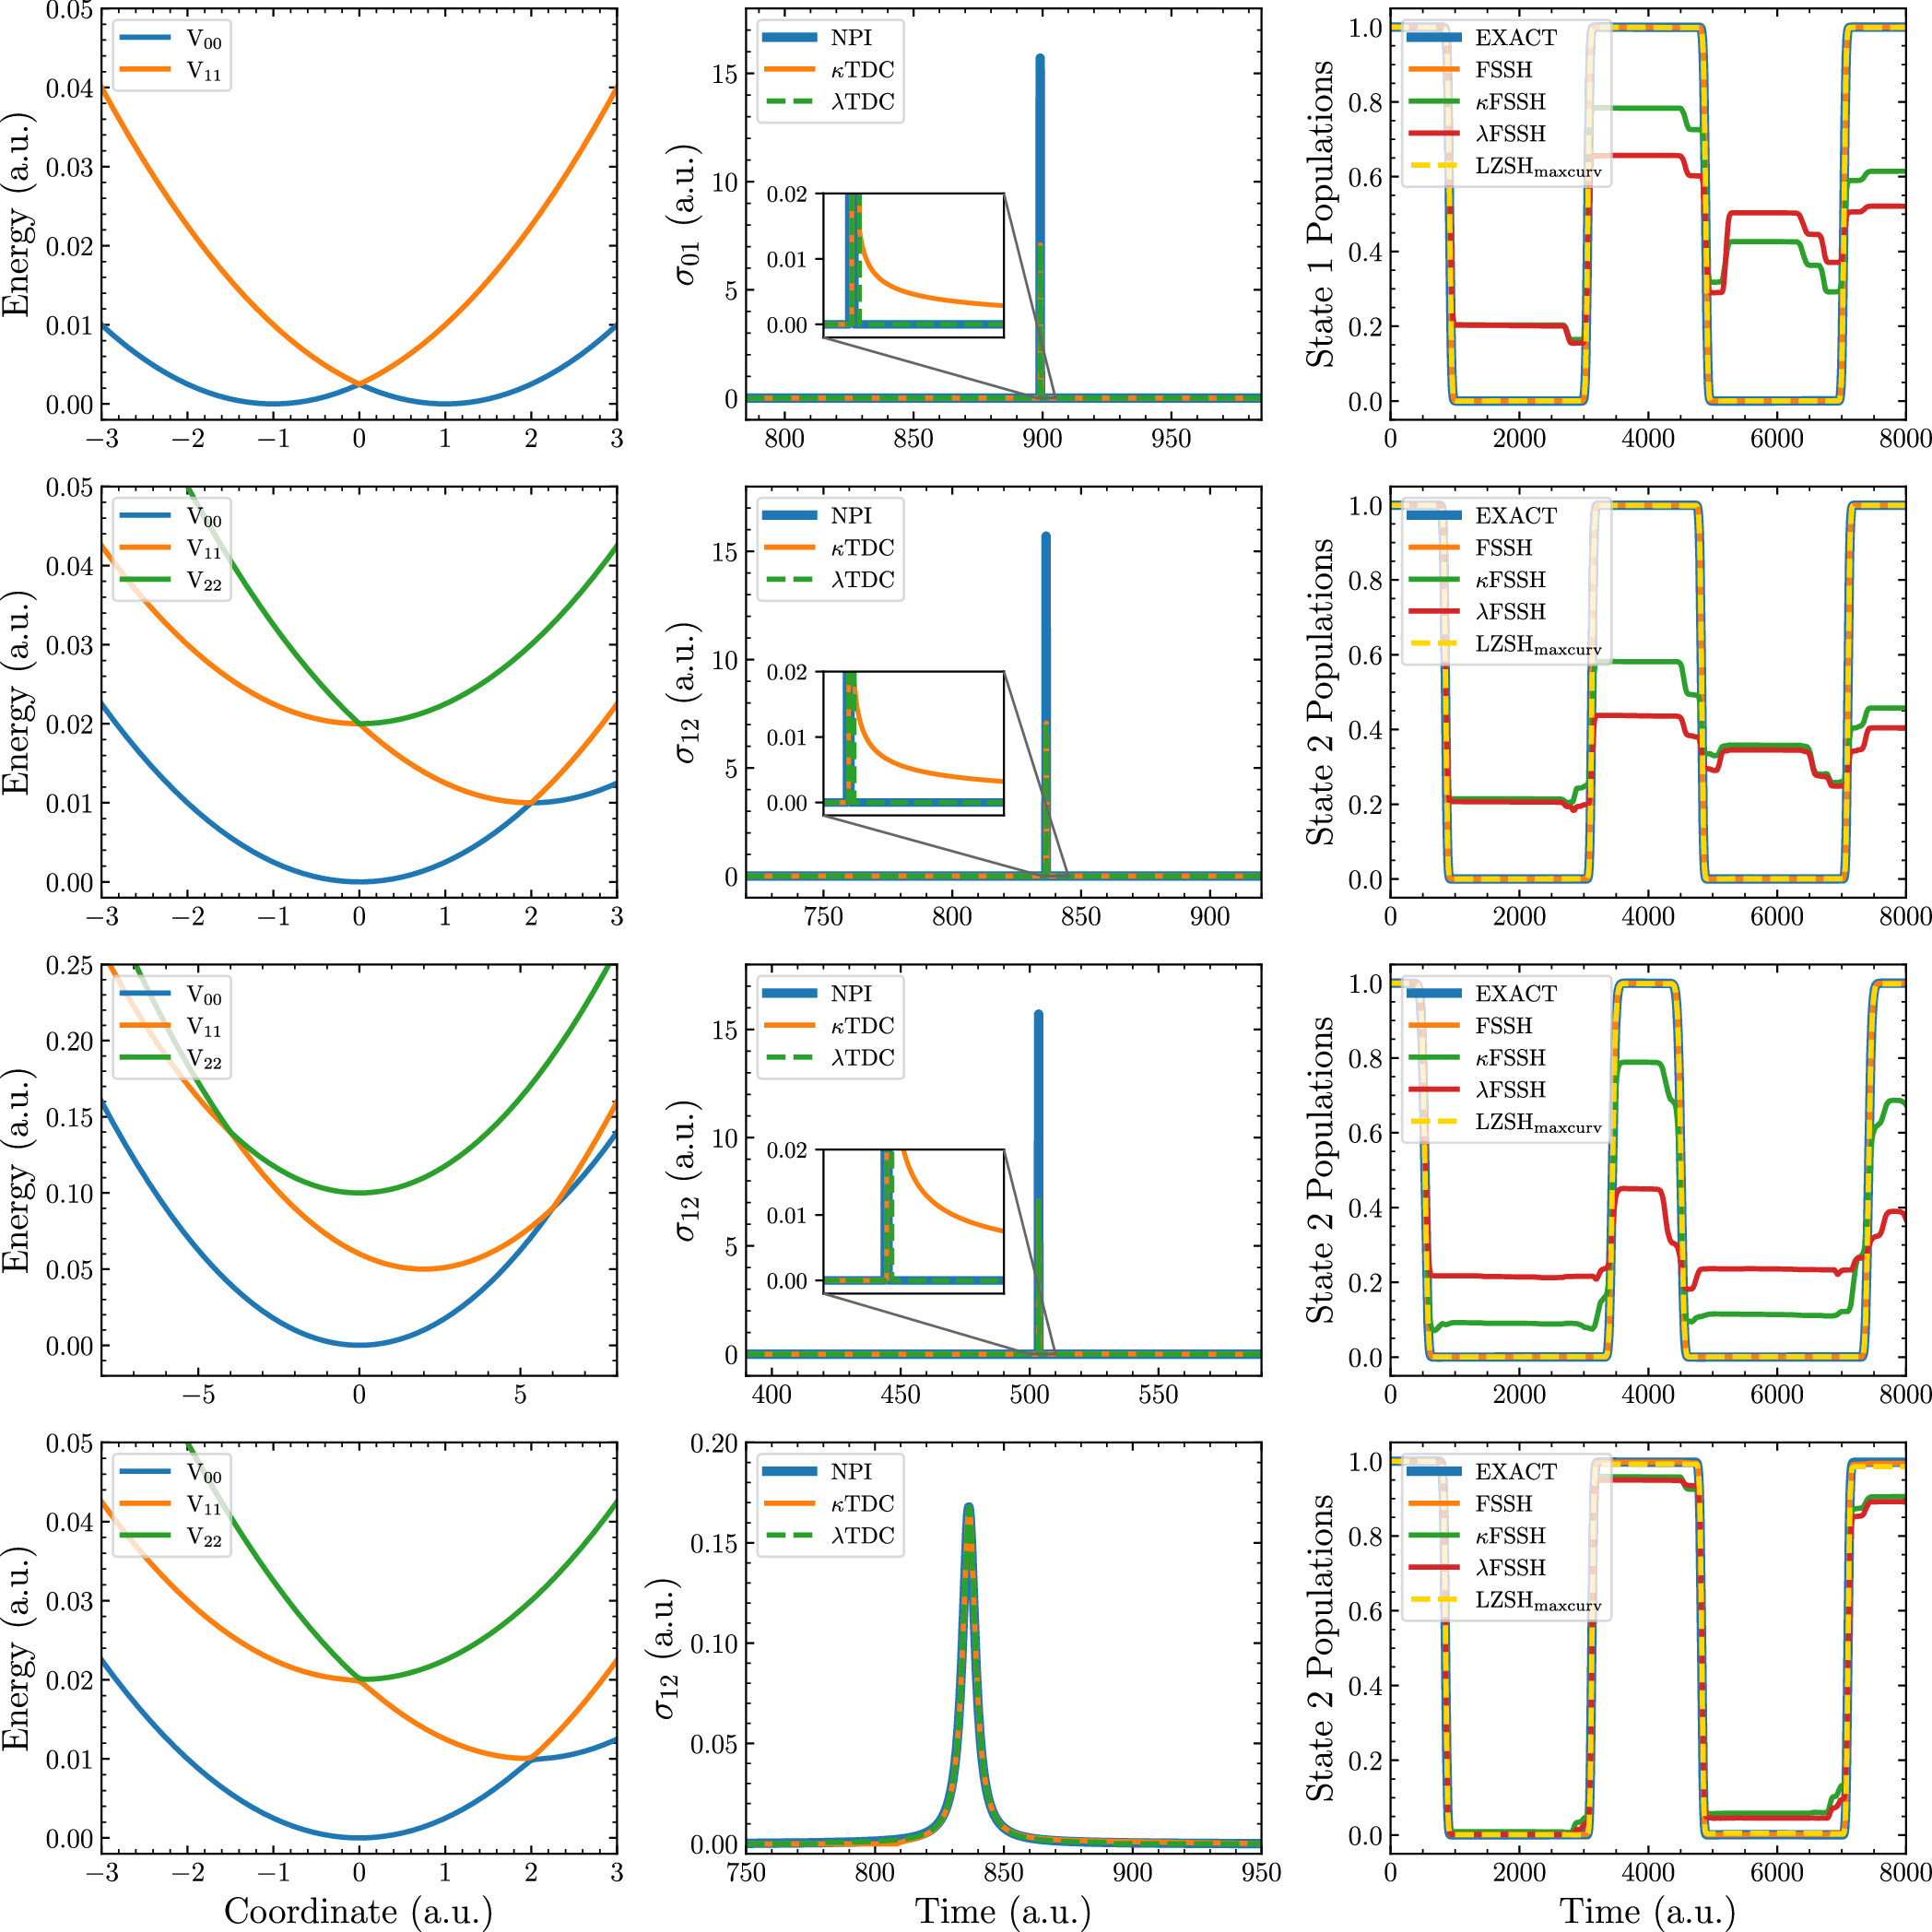
\includegraphics[width=\linewidth]{parts/02-Original_Research_and_Contributions/chapters/02-Primary_Scientific_Contributions/sections/images/images_large_ct5c01176_0004}
\caption{Nonadiabatic dynamics simulations on trivial crossing models. Reproduced from Ref.~\cite{10.1021/acs.jctc.5c01176} under \href{https://creativecommons.org/licenses/by/4.0}{CC BY 4.0}.}
\label{fig:curvature_trivial_crossing}
\end{figure}
\subsection{Vibronic Coupling Model of Uracil Cation}
Applying the algorithms to the 8-dimensional vibronic coupling model of the uracil cation, the failures of the $\kappa$\gls{fssh} method seen in 1D models are somewhat dampened, as seen in Fig.~\ref{fig:curvature_uracil}. It turns out that working in eight dimensions is actually quite forgiving for the algorithm, even if it is completely unforgiving for the human attempting to mentally visualize the crossing seams. \gls{fssh}, \gls{lzsh}, and $\kappa$\gls{fssh} all qualitatively capture the ultrafast relaxation. This suggests that the complex topology of multidimensional crossing seams can be more forgiving than strict 1D models. However, quantitative discrepancies remain visible: while the reference \gls{fssh} correctly predicts negligible population transfer to the $D_3$ state, the curvature-driven approaches inaccurately leak population into $D_3$, once again indicating a structural limitation in capturing the correct coupling mechanisms in densely packed state manifolds.
\begin{figure}[!ht]
\centering
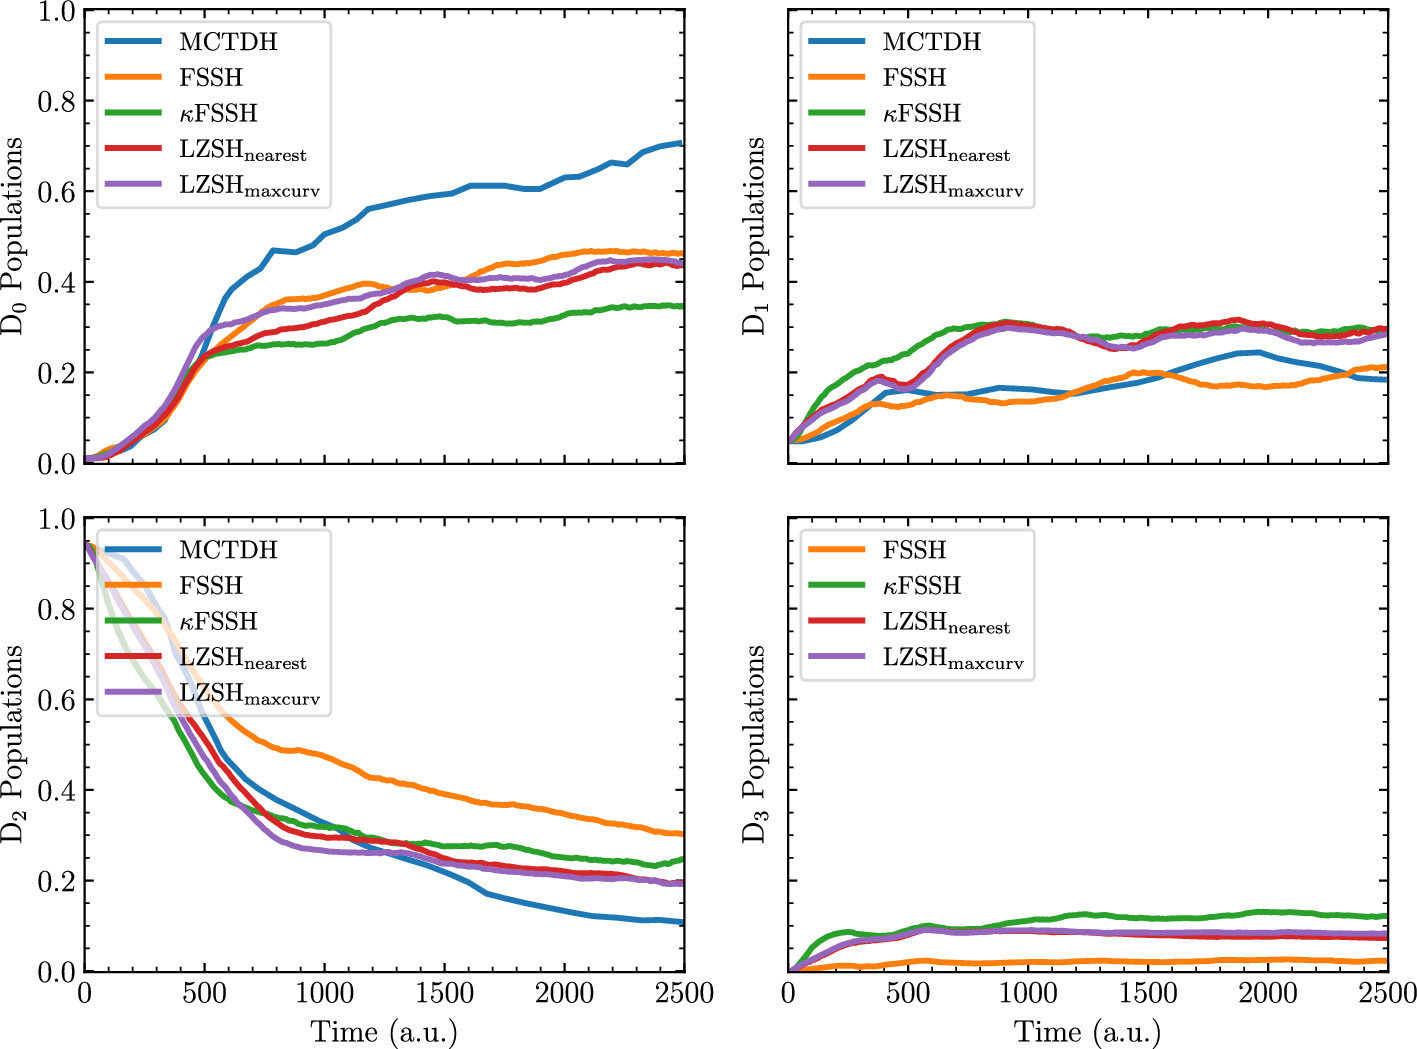
\includegraphics[width=\linewidth]{parts/02-Original_Research_and_Contributions/chapters/02-Primary_Scientific_Contributions/sections/images/images_large_ct5c01176_0005}
\caption{Nonadiabatic dynamics simulations on vibronic coupling model of uracil cation. Reproduced from Ref.~\cite{10.1021/acs.jctc.5c01176} under \href{https://creativecommons.org/licenses/by/4.0}{CC BY 4.0}.}
\label{fig:curvature_uracil}
\end{figure}
\subsection{Simulations on Realistic Systems}
The most severe limitations of curvature-driven methods emerge when applied to on-the-fly \textit{ab initio} simulations of real molecules like \textit{cis}-stilbene, \textit{trans}-azobenzene (Fig.~\ref{fig:curvature_stilbene}), and cyclobutanone. In these realistic systems, multireference electronic structure calculations (like OM3-MRCISD or CASSCF) frequently yield \glspl{pes} with small, localized discontinuities due to orbital rotations into the active space or state-averaging root flipping. 

Because the $\kappa$\gls{fssh} method depends directly on the second time-derivative of the energy gap ($\ddot{Z}_{ik}$), even a microscopic discontinuity in the \gls{pes} causes the numerical second derivative to explode. This translates into erratic spikes in the simulated \gls{tdc}, triggering continuous spurious hops and entirely corrupting the state populations. 

To salvage trajectory stability in such environments, this study introduced a novel discontinuity-blocking algorithm for the \gls{lzsh} method. When the \gls{lzsh} algorithm detects a minimum in the energy gap, it computes a ratio ($\alpha$) of the numerical second derivatives at the current and previous time steps. True avoided crossings exhibit smooth variations in curvature ($\alpha<0.3$), whereas discontinuities trigger abrupt changes ($\alpha>1.3$). By dynamically blocking hops when $\alpha>1.3$, the modified \gls{lzsh} algorithm successfully navigates rough \textit{ab initio} surfaces where $\kappa$\gls{fssh} fails, as evidenced by its strong agreement with standard \gls{fssh} in Fig.~\ref{fig:curvature_stilbene}.
\begin{figure}[!ht]
\centering
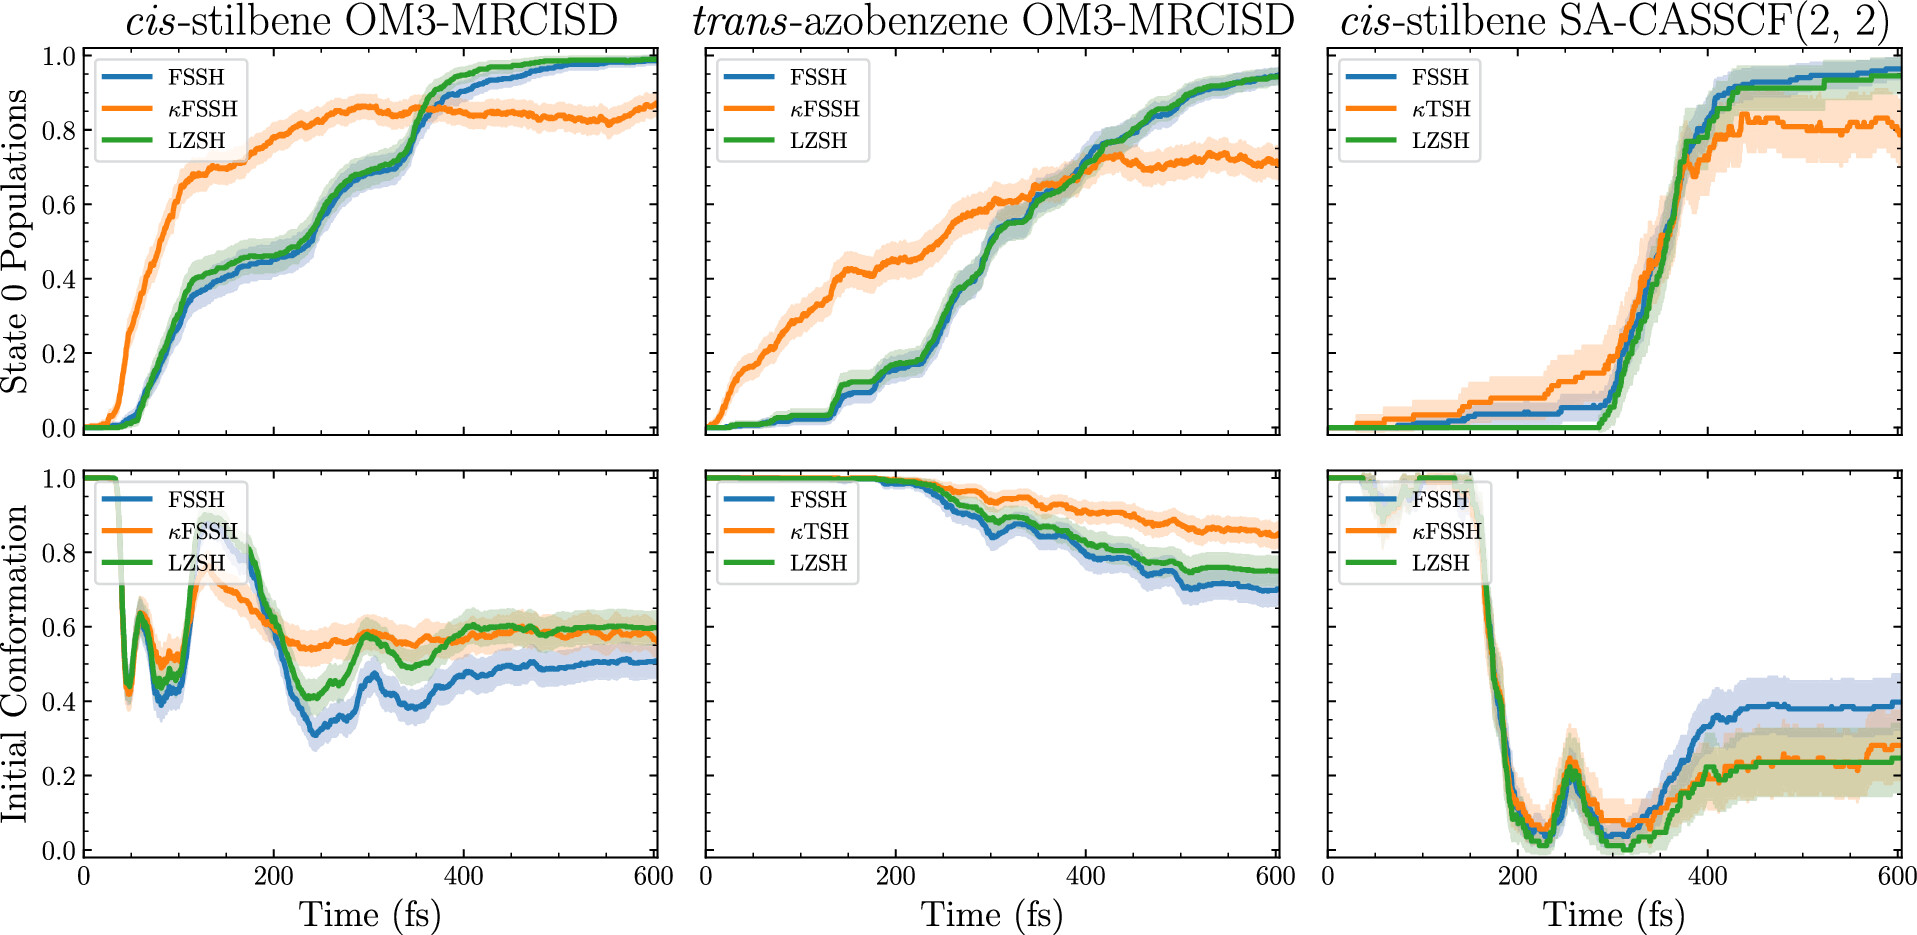
\includegraphics[width=\linewidth]{parts/02-Original_Research_and_Contributions/chapters/02-Primary_Scientific_Contributions/sections/images/images_large_ct5c01176_0006}
\caption{Nonadiabatic dynamics simulations on \textit{cis}-stilbene and \textit{trans}-azobenzene. Reproduced from Ref.~\cite{10.1021/acs.jctc.5c01176} under \href{https://creativecommons.org/licenses/by/4.0}{CC BY 4.0}.}
\label{fig:curvature_stilbene}
\end{figure}
\subsection{Conclusion}
The study presented here provides a comprehensive evaluation of the curvature-driven $\kappa$\gls{fssh} method against traditional \gls{fssh} and \gls{lzsh} approaches across a spectrum of model systems and realistic molecular simulations. Ultimately, we learned that while bypassing the need for \gls{nacv} by relying solely on the curvature of the adiabatic energy gap is an appealing shortcut, it suffers from significant limitations. In idealized 1D models, the $\kappa$\gls{fssh} method completely fails to reproduce correct state populations and \gls{tdc} values, particularly in systems with trivial crossings. More importantly, severe breakdowns also occur in realistic on-the-fly \textit{ab initio} simulations of molecules like \textit{cis}-stilbene and \textit{trans}-azobenzene, where the presence of discontinuities in the \glspl{pes} leads to erratic spikes in the \gls{tdc} and unphysical population transfer. In contrast, the traditional \gls{fssh} and \gls{lzsh} methods consistently outperform the curvature-driven approach in terms of state populations and \gls{tdc} values across all tested systems.

In the broader context of this thesis, these findings validate the numerical benchmarking and exact quantum dynamics framework (developed via the custom \textsc{Zinq} package) detailed in studies in Chapter~\ref{chp:supporting_numerical_studies}. Furthermore, to improve the \gls{lzsh} method's robustness in realistic \textit{ab initio} simulations, we introduced a novel discontinuity-blocking algorithm that successfully navigates rough \glspl{pes} where $\kappa$\gls{fssh} fails. Future research may focus on refining the curvature-driven algorithms to enhance their accuracy and reliability in nonadiabatic dynamics simulations, while also exploring specific applications where the $\kappa$\gls{fssh} method could still be useful despite its limitations.

This study provides two primary contributions to the application of nonadiabatic dynamics. First, they inform the computational chemistry community that algorithms relying on the curvature of the adiabatic energy gap are inherently incompatible with noisy or discontinuous \glspl{pes}, which are common in realistic \textit{ab initio} simulations. Second, it delivers a highly practical solution in the form of a discontinuity-blocking and 3-state-crossing-compatible variation of the \gls{lzsh} algorithm, which can be easily implemented in existing quantum chemistry codes to enhance the robustness of nonadiabatic dynamics simulations without the need for \gls{nacv}.
